%\Vorlesung 1
\part{Sortieren und Suchen}
\chapter{Bubblesort}


\begin{figure}[H]
\begin{center}
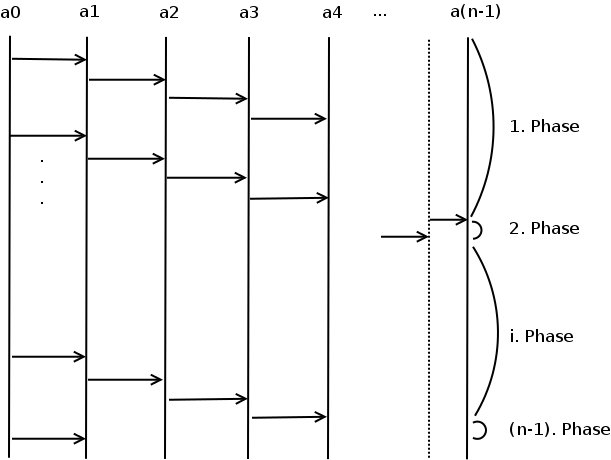
\includegraphics[width=0.8\linewidth]{01/Grafik/Bubblesort.png}
\caption{Bubblesort}
\end{center}
\end{figure}


\section{Pseudocode}
\begin{lstlisting}[style = pseudo]
void bubblesort (int[] a) {
  int n = a.length;
  for (int i = 1; i < n; i++) {
    for (int j = 0; j < n-i; j++) {
      if (a[j] < a[j+1])
        swap (a, j, j+1);
    }
  }
}
\end{lstlisting}
\paragraph{Schleifen-Invariante:} Nach dem Ablauf der i-ten Phase gilt:
\begin{center}
	Die Feldpositionen n-i,\ldots,n enthalten die korrekt sortierten Feldelemente
\end{center}
\paragraph{Beweis} durch Induktion nach i $\overset{i=n-1}{\Longrightarrow}$ Sortierung am Ende korrekt.


\pagebreak

\section{Laufzeitanalyse}

$T(n) =$ Zahl der durchgeführten Elementvergleiche für eine Eingabemenge von n Elementen\\

\begin{tabular}{rcc}
	1.&Phase & n-1 \\
	2.&Phase & n-2 \\
	3.&Phase & n-3 \\
	 & $\vdots$ &  \\
	i.& Phase & n-i \\
	 & $\vdots$ &  \\
	(n-1).&Phase & n-(n-1)=1 \\ \hline
	\multicolumn{3}{c}{$1+2+3+\ldots+(n-1)$}
\end{tabular}
\[ T(n)=\sum_{i=1}^{n-1} i = \frac{n(n-1)}{2}\in O(n^2) \]
\begin{tabular}{c|c}
	$n$ & $T_{real}$ \\ \hline
	$2^{10}$ & 8ms \\
	$2^{11}$ & 11ms \\
	$2^{12}$ & 26ms \\
	$\vdots$ &  \\
	$2^{16}$ & 5,819s \\
	$2^{17}$ & 23,381s \\
	$\vdots$ &  \\
	$2^{20}$ & 16min \\
	$\vdots$ &  \\
	$2^{26}$ & 52d 
\end{tabular}
\[ T_{real}(n)\approx cn^2~~ c\approx10^{-6}\]
\[T_{real} (2n) \approx c \cdot (2n)^2 = 4 cn^2 = 4T_{real}(n) \]
\[\frac{T_{real}(2n)}{T_{real}(n)} = 4 \]



\chapter{Heapsort}
\label{sec:heapsort}

\paragraph{z.B.} \begin{tabular}{ccccccccccccccc}
	21&6&4&7&12&5&3&11&14&17&19&8&9&10&42
\end{tabular}

%hier dürfen gerne noch die einzelnen Schritte als Grafik eingefügt werden

\section{Skizze}
\begin{figure}[h]
%\begin{center}
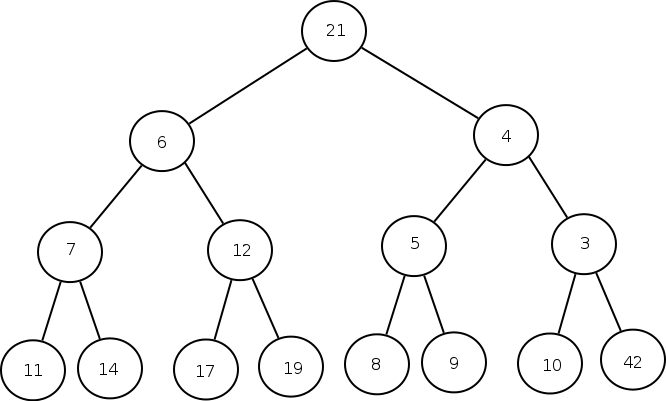
\includegraphics[width=0.3\linewidth]{01/Grafik/heap1.png}
\captionsetup{labelsep=space,justification=justified,singlelinecheck=off}
\caption{Heapsort (Ausgangssituation)}
%\end{center}
\end{figure}


\subsection{Indices innerhalb der Baumstruktur}
\begin{flalign*}
&\lfloor \frac{i-1}{2} \rfloor&
\end{flalign*}

\begin{figure}[h]
\vspace{-45pt}
\hspace{35pt}
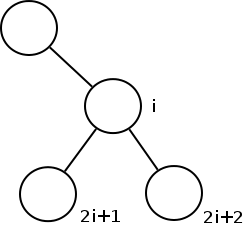
\includegraphics[width=0.2\linewidth]{01/Grafik/HeapAufbau.png}
\caption{Indices}
\end{figure}


\section{Heap-Eigenschaft}

\begin{figure}[h]
\begin{center}
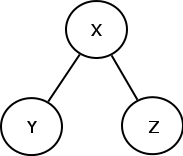
\includegraphics[width=0.2\linewidth]{01/Grafik/HeapEigenschaft.png}\\
$x \geq y$\\
$x \geq z$
\caption{Heap-Eigenschaft}
\end{center}
\end{figure}


\section{Idee}
\paragraph{Phase 1} Stelle die Heap-Eigenschaft überall her\\
$\Rightarrow$ größtes Element steht in der Wurzel
\paragraph{Phase 2} Tausche Wurzel mit letztem Feldelement\\
(z.B. 42 mit 3)\\
- Entferne letztes Feldelement aus dem Baum\\
- Gehe erneut zu Phase 1
